\documentclass{article}


\usepackage{neurips_2025}
% \usepackage[final]{neurips_2025}


\usepackage{listings}     % For ASCII-art / code blocks
\usepackage{booktabs}     % Nicer tables
\usepackage{array}        % Column types
\usepackage{tabularx}     % Automatic column width
\usepackage{enumitem}     % Compact lists



\usepackage{comment}

\usepackage[utf8]{inputenc}
\usepackage[T1]{fontenc}
\usepackage{textcomp}
\usepackage[english]{babel} 
\usepackage{url}
\usepackage{graphicx}


\usepackage{hyperref}       % hyperlinks
\usepackage{amsfonts}       % blackboard math symbols
\usepackage{nicefrac}       % compact symbols for 1/2, etc.
\usepackage{microtype}      % microtypography
\usepackage{xcolor}         % colors



\DeclareUnicodeCharacter{00A0}{~}      % Non-breaking space
\DeclareUnicodeCharacter{00A1}{\textexclamdown}
\DeclareUnicodeCharacter{00A2}{\textcent}
\DeclareUnicodeCharacter{00A3}{\textsterling}
\DeclareUnicodeCharacter{00A5}{\textyen}
\DeclareUnicodeCharacter{00A7}{\S}
\DeclareUnicodeCharacter{00A8}{\"{}}
\DeclareUnicodeCharacter{00A9}{\textcopyright}
\DeclareUnicodeCharacter{00AA}{\textordfeminine}
\DeclareUnicodeCharacter{00AB}{\guillemotleft}
\DeclareUnicodeCharacter{00AC}{\textlnot}
\DeclareUnicodeCharacter{00AD}{}       % Soft hyphen
\DeclareUnicodeCharacter{00AE}{\textregistered}
\DeclareUnicodeCharacter{00AF}{\={}}   % Macron

\DeclareUnicodeCharacter{00B0}{\textdegree}
\DeclareUnicodeCharacter{00B1}{\textpm}
\DeclareUnicodeCharacter{00B2}{\textsuperscript{2}}
\DeclareUnicodeCharacter{00B3}{\textsuperscript{3}}
\DeclareUnicodeCharacter{00B4}{\'{}}   % Acute accent
\DeclareUnicodeCharacter{00B5}{\textmu}
\DeclareUnicodeCharacter{00B6}{\P}
\DeclareUnicodeCharacter{00B7}{\textperiodcentered}
\DeclareUnicodeCharacter{00B8}{\c{}}   % Cedilla
\DeclareUnicodeCharacter{00B9}{\textsuperscript{1}}
\DeclareUnicodeCharacter{00BA}{\textordmasculine}
\DeclareUnicodeCharacter{00BB}{\guillemotright}
\DeclareUnicodeCharacter{00BC}{\textonequarter}
\DeclareUnicodeCharacter{00BD}{\textonehalf}
\DeclareUnicodeCharacter{00BE}{\textthreequarters}
\DeclareUnicodeCharacter{00BF}{\textquestiondown}

% Accented letters (common in names)
\DeclareUnicodeCharacter{00C0}{\`A}
\DeclareUnicodeCharacter{00C1}{\'A}
\DeclareUnicodeCharacter{00C2}{\^A}
\DeclareUnicodeCharacter{00C3}{\~A}
\DeclareUnicodeCharacter{00C4}{\"A}
\DeclareUnicodeCharacter{00C5}{\AA}
\DeclareUnicodeCharacter{00C6}{\AE}
\DeclareUnicodeCharacter{00C7}{\c{C}}
\DeclareUnicodeCharacter{00C8}{\`E}
\DeclareUnicodeCharacter{00C9}{\'E}
\DeclareUnicodeCharacter{00CA}{\^E}
\DeclareUnicodeCharacter{00CB}{\"E}
\DeclareUnicodeCharacter{00CC}{\`I}
\DeclareUnicodeCharacter{00CD}{\'I}
\DeclareUnicodeCharacter{00CE}{\^I}
\DeclareUnicodeCharacter{00CF}{\"I}
\DeclareUnicodeCharacter{00D1}{\~N}
\DeclareUnicodeCharacter{00D2}{\`O}
\DeclareUnicodeCharacter{00D3}{\'O}
\DeclareUnicodeCharacter{00D4}{\^O}
\DeclareUnicodeCharacter{00D5}{\~O}
\DeclareUnicodeCharacter{00D6}{\"O}
\DeclareUnicodeCharacter{00D8}{\O}
\DeclareUnicodeCharacter{00D9}{\`U}
\DeclareUnicodeCharacter{00DA}{\'U}
\DeclareUnicodeCharacter{00DB}{\^U}
\DeclareUnicodeCharacter{00DC}{\"U}
\DeclareUnicodeCharacter{00DD}{\'Y}
\DeclareUnicodeCharacter{00DF}{\ss}

\DeclareUnicodeCharacter{00E0}{\`a}
\DeclareUnicodeCharacter{00E1}{\'a}
\DeclareUnicodeCharacter{00E2}{\^a}
\DeclareUnicodeCharacter{00E3}{\~a}
\DeclareUnicodeCharacter{00E4}{\"a}
\DeclareUnicodeCharacter{00E5}{\aa}
\DeclareUnicodeCharacter{00E6}{\ae}
\DeclareUnicodeCharacter{00E7}{\c{c}}
\DeclareUnicodeCharacter{00E8}{\`e}
\DeclareUnicodeCharacter{00E9}{\'e}
\DeclareUnicodeCharacter{00EA}{\^e}
\DeclareUnicodeCharacter{00EB}{\"e}
\DeclareUnicodeCharacter{00EC}{\`i}
\DeclareUnicodeCharacter{00ED}{\'i}
\DeclareUnicodeCharacter{00EE}{\^i}
\DeclareUnicodeCharacter{00EF}{\"i}
\DeclareUnicodeCharacter{00F1}{\~n}
\DeclareUnicodeCharacter{00F2}{\`o}
\DeclareUnicodeCharacter{00F3}{\'o}
\DeclareUnicodeCharacter{00F4}{\^o}
\DeclareUnicodeCharacter{00F5}{\~o}
\DeclareUnicodeCharacter{00F6}{\"o}
\DeclareUnicodeCharacter{00F8}{\o}
\DeclareUnicodeCharacter{00F9}{\`u}
\DeclareUnicodeCharacter{00FA}{\'u}
\DeclareUnicodeCharacter{00FB}{\^u}
\DeclareUnicodeCharacter{00FC}{\"u}
\DeclareUnicodeCharacter{00FD}{\'y}
\DeclareUnicodeCharacter{00FF}{\"y}

% Common punctuation
\DeclareUnicodeCharacter{2013}{--}       % en dash
\DeclareUnicodeCharacter{2014}{---}      % em dash
\DeclareUnicodeCharacter{2018}{`}        % left single quote
\DeclareUnicodeCharacter{2019}{'}        % right single quote / apostrophe
\DeclareUnicodeCharacter{201C}{``}       % left double quote
\DeclareUnicodeCharacter{201D}{''}       % right double quote
\DeclareUnicodeCharacter{2022}{\textbullet}
\DeclareUnicodeCharacter{2026}{\ldots}   % ellipsis

% Currency and symbols
\DeclareUnicodeCharacter{20AC}{\euro}    % euro
\DeclareUnicodeCharacter{2122}{\texttrademark}



\title{AgentSight: System-Level Observability for AI Agents Using eBPF}



\author{%
  Yusheng Zheng$^{1}$ \\
  \texttt{yzhen165@ucsc.edu} \\
  \And
  Yanpeng Hu$^{2}$ \\
  \texttt{huyp@shanghaitech.edu.cn} \\
  \And
  Tong Yu$^{3}$ \\
  \texttt{yt.xyxx@gmail.com} \\
  \And
  Andi Quinn$^{1}$ \\
  \texttt{aquinn1@ucsc.edu} \\
  \And
  \multicolumn{4}{c}{$^{1}$UC Santa Cruz, Santa Cruz, CA, USA} \\
  \multicolumn{4}{c}{$^{2}$ShanghaiTech University, Shanghai, China} \\
  \multicolumn{4}{c}{$^{3}$eunomia-bpf Community, China}
}

\sloppy
\begin{document}


\maketitle


\begin{abstract}
    Modern software infrastructure increasingly relies on LLM agents for development and maintenance, such as Claude Code and Gemini-cli. However, these AI agents differ fundamentally from traditional deterministic software, posing a significant challenge to conventional monitoring and debugging. This creates a critical semantic gap: existing tools observe either an agent's high-level intent (via LLM prompts) or its low-level actions (e.g., system calls), but cannot correlate these two views. This blindness makes it difficult to distinguish between benign operations, malicious attacks, and costly failures. We introduce AgentSight, an AgentOps observability framework that bridges this semantic gap using a hybrid approach. Our approach, \emph{boundary tracing}, monitors agents from outside their application code at stable system interfaces using eBPF. AgentSight intercepts TLS-encrypted LLM traffic to extract semantic intent, monitors kernel events to observe system-wide effects, and causally correlates these two streams across process boundaries using a real-time engine and secondary LLM analysis. This instrumentation-free technique is framework-agnostic, resilient to rapid API changes, and incurs less than 3\% performance overhead. Our evaluation shows AgentSight detects prompt injection attacks, identifies resource-wasting reasoning loops, and reveals hidden coordination bottlenecks in multi-agent systems. AgentSight is released as an open-source project at \url{https://github.com/eunomia-bpf/agentsight}.
\end{abstract}



\maketitle
\pagestyle{plain}


\section{Introduction}

AI agents violate the fundamental assumptions of software monitoring. Unlike traditional programs with predictable execution paths, agents combine Large Language Models (LLMs) with autonomous tool use, enabling them to dynamically generate code, spawn arbitrary subprocesses, and alter their behavior based on natural language goals. This paradigm shift creates a critical \textbf{semantic gap}: the chasm between an agent's high-level \emph{intent} and its low-level \emph{system actions}. Consider an agent tasked with code refactoring that, due to a malicious prompt, instead injects a backdoor. An application-level monitor might see a successful "execute script" tool call, while a system monitor sees a \texttt{git commit} process writing to a file. Neither can bridge the gap to understand that a benign intention has been twisted into a malicious action, rendering them effectively blind.

This semantic gap makes it impossible for existing observability tools to distinguish between benign operations and catastrophic failures. Current approaches fall into two categories, each blind to one side of the gap. \textbf{Application-level instrumentation}, found in frameworks like LangChain~\cite{langchain} and AutoGen~\cite{autogen}, uses hooks and logs to capture the agent's reasoning and tool selections. While these tools see the \emph{intent}, they are fundamentally limited. They are brittle, requiring constant updates to keep pace with framework APIs that see dozens of breaking changes monthly. More critically, they are easily bypassed; a single shell command spawned by an agent escapes their view, breaking the chain of visibility. They operate on a flawed trust model, assuming a cooperative agent that will not be compromised or exhibit emergent, unlogged behaviors.

On the other side, \textbf{generic system-level monitoring} tools see the \emph{actions}. They can track every system call, file access, and network connection. However, they lack all semantic context. To them, an agent writing a data analysis script to \texttt{/tmp} is indistinguishable from a compromised agent writing a malicious payload to the same location. Without understanding the preceding LLM instructions—the \emph{why} behind the \emph{what}—their stream of low-level events is meaningless noise, leading to an overwhelming volume of false positives and inactionable alerts.

We propose \emph{boundary tracing} as a novel observability paradigm designed specifically to bridge this semantic gap. Our key insight is that while agent internals and frameworks are volatile, the interfaces through which they interact with the world—the kernel for system operations and the network for communication—are stable and unavoidable. By monitoring from outside the application at these tamper-proof boundaries, we can simultaneously capture an agent's high-level intent and its low-level system effects, creating a complete, correlated picture of its behavior. This approach replaces the broken trust model of instrumentation with enforced, comprehensive observation.

This paper presents AgentSight, a system that realizes the boundary tracing paradigm using eBPF technology. AgentSight intercepts TLS-encrypted LLM traffic to understand semantic intent and monitors kernel events to observe system-wide effects. Its core contribution is its ability to \textbf{causally correlate these two streams across process boundaries}, linking a specific LLM response to the sequence of system calls it triggers, even in subprocesses. This instrumentation-free technique is framework-agnostic and incurs less than 3\% performance overhead. Our evaluation shows AgentSight detects sophisticated prompt injection attacks with 92\% confidence, automatically identifies resource-wasting reasoning loops, and reveals hidden bottlenecks in multi-agent systems.

\textbf{This paper makes three primary contributions:}

\begin{enumerate}
\item \textbf{Boundary Tracing Paradigm}: We introduce boundary tracing as a principled approach to AI agent observability that bridges the semantic gap by monitoring at stable system interfaces.

\item \textbf{System-Level Correlation}: We present AgentSight's eBPF-based implementation that causally correlates TLS-intercepted LLM communications with kernel-level operations across process boundaries.

\item \textbf{Production Validation}: We demonstrate AgentSight's effectiveness in detecting prompt injection attacks (92\% confidence), reasoning loops, and multi-agent coordination failures with sub-3\% overhead.
\end{enumerate}

\section{Background and Related Work}

This section outlines LLM agent architecture, reviews existing observability work to highlight the semantic gap, and introduces eBPF as our foundational technology.

% \subsection{LLM Agent Architecture}
% AI agents represent a new class of software systems that combine language models with environmental interactions. These systems typically consist of three core components: (1) an LLM backend that provides reasoning capabilities, (2) a tool execution framework that enables system interactions, and (3) a control loop that orchestrates prompts, tool calls, and state management. Popular frameworks such as LangChain~\cite{langchain}, AutoGen~\cite{autogen}, cursor agent\cite{cursor}, genimi-cli\cite{geminicli} and Claude Code\cite{claudecode} implement variations of this architecture and are widely used in production. The key characteristic distinguishing AI agents from traditional software is their ability to dynamically construct execution plans based on natural language objectives (e.g., an agent tasked with "analyze this dataset" might autonomously decide to install packages, write analysis scripts, execute them, and interpret results), all without predetermined logic paths. This flexibility comes from the LLM's ability to generate arbitrary code and command sequences.

\subsection{LLM Agent Architecture}
The agentic systems described in the introduction are typically implemented using a common architecture. These systems consist of three core components: (1) an LLM backend for reasoning, (2) a tool execution framework for system interactions, and (3) a control loop that orchestrates prompts, tool calls, and state management. Popular frameworks such as LangChain~\cite{langchain}, AutoGen~\cite{autogen}, Cursor Agent\cite{cursor}, Gemini-CLI\cite{geminicli} and Claude Code\cite{claudecode} all implement variations of this model. This architecture is what enables agents to dynamically construct and execute complex plans (e.g., autonomously writing and running a script to analyze a dataset) based on high-level natural language objectives. Multi-agent LLM systems have also emerged for software development, collaborative task-solving, simulating social behaviors in virtual worlds, and other tasks~\cite{guo2024survey,tran2025survey}.

\subsection{Observability for LLM Agent}

Existing approaches are siloed on one side of the semantic gap. Intent-side observability, supported by industry tools like Langfuse, LangSmith, and Datadog~\cite{Maierhofer2025Langfuse, langfuse, langsmith, Datadog2023Agents, helicone} and is unifying by standards from the OpenTelemetry GenAI working group~\cite{Liu2025OTel,Bandurchin2025Uptrace} and acadamics conceptual taxonomies~\cite{Dong2024AgentOps, Moshkovich2025Pipeline} under the AgentOps concept, excels at tracing application-level events but is fundamentally blind to out-of-process system \emph{actions}. Conversely, action-side observability with tools like Falco and Tracee~\cite{falco, tracee} offers comprehensive visibility into system calls but lacks the semantic context to understand an agent's \emph{intent}, failing to distinguish a benign task from a malicious one. A parallel line of research into reasoning-level and interpretability aims to make the agent's internal thought processes more transparent by reconstructing cognitive traces~\cite{Rombaut2025Watson} or enabling explanatory dialogues~\cite{Kim2025AgenticInterp}, but these work mainly focus on the llm itself, does not bridge the gap between the agent's internal reasoning and its external, low-level effects on the system.

\subsection{extended Berkeley Packet Filter (eBPF)}

To bridge the semantic gap, our approach requires a technology that can safely and efficiently observe both network communication and kernel activity. eBPF (extended Berkeley Packet Filter) is a fundamental advancement in kernel programmability that provides precisely this capability~\cite{brendangregg}. Originally designed for packet filtering, eBPF has evolved into a general-purpose, in-kernel virtual machine that powers modern observability and security tools~\cite{ebpfio,cilium}, and not limited to Linux\cite{zheng2025extending, windows-ebpf}. For AI agent observability, eBPF is uniquely suited because it allows observation at the exact boundaries where agents interact with the world, enabling both TLS interception for semantic \emph{intent} and syscall monitoring for system \emph{actions} with minimal overhead. Critically, its kernel-enforced safety guarantees, including verified termination and memory safety, make it ideal for production environments and provide a stable foundation for our solution~\cite{kerneldoc}.


% \subsection{Observability for LLM Agent}


% Observability has historically been critical for building trustworthy and maintainable software systems. Early research, such as Shortliffe et al. pioneering work on the MYCIN expert system in 1975, highlighted the importance of transparent reasoning, establishing foundational concepts for interpreting and monitoring agent-based systems~\cite{Shortliffe1975Mycin}. With the advent of modern large language model (LLM)-driven systems, the complexity and autonomy of AI agents have dramatically increased, amplifying the necessity for enhanced observability. Contemporary AI agents frequently exhibit emergent and non-deterministic behaviors, making traditional observability approaches insufficient for ensuring system reliability, safety, and correctness~\cite{Dong2024AgentOps,Noble2025IBM}.

% Recent work in the domain, such as the \emph{AgentOps} taxonomy developed by Dong et al., underscores the necessity of capturing detailed artifacts such as prompts, tool invocations, and memory interactions as first-class telemetry data for comprehensive observability~\cite{Dong2024AgentOps}. Moshkovich and Zeltyn expand upon this perspective by proposing a structured six-stage automation pipeline that leverages observational data to enable automated analysis and mitigation strategies, thus addressing critical operational challenges when observability data is incomplete or unavailable in production scenarios~\cite{Moshkovich2025Pipeline}.

% Furthermore, frameworks such as \emph{Watson} proposed by Rombaut et al. delve deeper into cognitive-level observability by reconstructing an LLM's implicit reasoning traces, thereby making the agent's internal cognitive processes explicitly visible~\cite{Rombaut2025Watson}. Complementing this, Kim et al. advocate for \emph{agentic interpretability}, wherein LLMs engage in interactive dialogues, actively explaining their reasoning and behaviors to users, effectively positioning the model itself as a cooperative participant in achieving greater transparency and observability~\cite{Kim2025AgenticInterp}.

% From an industry perspective, emerging standards such as those developed by the OpenTelemetry GenAI working group seek to unify observability practices by establishing common semantic conventions for tracing and logging agent actions across diverse frameworks~\cite{Liu2025OTel,Bandurchin2025Uptrace}. Additionally, tools like Langfuse and Datadog provide practical platforms for capturing detailed trace information and visualizing multi-agent workflows, enhancing developers' ability to diagnose and address complex agent interactions effectively~\cite{Maierhofer2025Langfuse,Datadog2023Agents}.

% In sum, the evolving landscape of AI agent observability highlights the critical need for advanced, robust, and integrated observability solutions that accommodate the unique challenges posed by autonomous and dynamically evolving agent behaviors.

% Despite its recognized importance, existing approaches to observability are insufficient due to the special characteristics of AI agents. The autonomy of AI agents creates a fundamental challenge that invalidates traditional monitoring paradigms: the \textbf{semantic gap}. This gap is the chasm between an agent's high-level, semantic \emph{intent} (the "why," captured in LLM interactions) and its low-level system \emph{actions} (the "what," observed as system calls). This chasm is created by two core agent behaviors: \textbf{Dynamic Execution Paths}, where an agent's operational sequence emerges from non-deterministic reasoning, and \textbf{Cross-Boundary Interactions}, where agents spawn subprocesses (\texttt{bash}, \texttt{curl}, \texttt{git}) that escape the monitoring scope of the parent process. 

% The danger of the unbridged semantic gap is not only theoretical. It manifests in significant reliability and security risks, as demonstrated by these real-world failure scenarios. In an \textbf{Unintended System Modification} incident, an AI agent tasked with code review misinterprets its instructions and begins modifying the production codebase. The semantic gap is exposed when application-level tools see the benign \emph{intent} ("review code") but are completely blind to the destructive system \emph{actions} (\texttt{git commit} and file modifications) occurring in a subprocess. A \textbf{Costly Reasoning Loop} occurs when a data analysis agent enters an infinite cycle calling expensive LLM APIs to solve an impossible problem, consuming thousands of dollars. Framework logs reveal the \emph{action} (high volume of API calls) but provide no insight into the semantic \emph{intent}, which is a looping pattern of thought, making it impossible to distinguish between productive work and a costly failure mode without bridging the gap. In a \textbf{Cross-Process Exploitation}, an agent compromised via prompt injection writes a malicious shell script to \texttt{/tmp} and executes it. The semantic gap here is critical as system monitors see the file-write and process-execution \emph{actions}, but without linking them to the malicious \emph{intent} from the prompt, they appear as benign, uncorrelated events, and only by bridging the gap can the full attack narrative be reconstructed. These incidents exemplify a new threat model unique to AI agents, where the disconnect between intent and action can lead to prompt injection attacks, goal drift, and unintended capability escalation.

% Because of this gap, observing only the intent or only the action is insufficient and misleading, demanding a new approach that can holistically link the two.

% \textbf{SDK-Based and Proxy-Based Instrumentation} solutions like LangSmith~\cite{langsmith}, Langfuse~\cite{langfuse}, and Helicone~\cite{helicone} operate on the \textbf{intent side} of the gap. They excel at capturing LLM prompts, responses, and tool choices. However, they are blind to any system \textbf{actions} that occur outside the instrumented framework, such as operations within a spawned shell script. Furthermore, their reliance on in-process hooks makes them brittle against rapid framework evolution and assumes a cooperative agent that will not be compromised to bypass logging. Noble et al.~\cite{Noble2025IBM} further illustrate these limitations, noting SDK-based observability's inability to reliably capture real-time malicious intent or system-level anomalies.

% \textbf{Generic System-Level Monitoring} tools like Falco~\cite{falco} and Tracee~\cite{tracee} operate on the \textbf{action side}. They provide comprehensive visibility into every system call and process execution but lack all semantic context. To these tools, an agent writing a file is just a file write; they cannot determine the \textbf{intent} behind it. As demonstrated in the exploitation scenario, they can report that a script was executed from \texttt{/tmp}, but cannot link this action back to the agent's reasoning, failing to distinguish a malicious attack from a legitimate task.

% Furthermore, reasoning-level observability remains underexplored. Rombaut et al.~\cite{Rombaut2025Watson} highlight the critical value of cognitive observability, where agent reasoning traces and implicit chains-of-thought are reconstructed for debugging, an aspect typically missed by conventional monitoring.

% No existing solution can simultaneously capture semantic intent and system actions, maintain visibility across process boundaries, and remain resilient to framework changes. This critical failure to bridge the semantic gap motivates our novel approach.

% % \begin{tikzpicture}[
%     % Global settings for a more compact layout
%     node distance=2mm and 5mm,
%     % --- STYLES ---
%     outerbox/.style={
%         draw, 
%         rectangle, 
%         minimum width=9cm, 
%         minimum height=10.5cm, 
%         line width=0.5pt
%     },
%     innerbox/.style={
%         draw, 
%         rectangle, 
%         minimum width=8cm, 
%         line width=0.5pt, 
%         fill=gray!5
%     },
%     boxtitle/.style={
%         font=\small\bfseries, 
%         text centered
%     },
%     boxsubtitle/.style={
%         font=\small\itshape, 
%         text centered, 
%         text width=6.5cm
%     },
%     listtext/.style={
%         font=\small, 
%         align=left
%     },
%     boundarytext/.style={
%         font=\small, 
%         fill=white, % White fill to sit cleanly over the line
%         inner sep=2pt
%     },
%     sidelabel/.style={
%         font=\small\itshape, 
%         align=left
%     },
%     boundaryline/.style={
%         draw, 
%         double, 
%         thick, 
%         gray!80
%     },
%     vertical_arrow/.style={
%         <->, % Bidirectional arrow
%         thick,
%         >=latex % Arrowhead style
%     }
% ]

% % 1. Main outer box and its title
% \node[outerbox] (main) {};
% \node[boxtitle, anchor=north, yshift=-4mm] at (main.north) {System Environment};
% \node[boxsubtitle, below=1mm of main.north] at (main.north) {(Operating System, Containers, Services)};

% % 2. Top inner box (Agent Runtime)
% \node[innerbox, minimum height=3cm, anchor=north, yshift=-1.8cm] (agent) at (main.north) {};
% \node[boxtitle, anchor=north, yshift=-4mm] at (agent.north) {Agent Runtime Framework};
% \node[boxsubtitle, anchor=north, yshift=-9mm] at (agent.north) {(LangChain, AutoGen, Claude Code)};
% \node[listtext, anchor=center, yshift=-4mm] at (agent.center) {
%     \textbullet~Prompt orchestration \\
%     \textbullet~Tool execution logic \\
%     \textbullet~State management
% };

% % 3. Bottom inner box (LLM Service)
% \node[innerbox, minimum height=1.6cm, anchor=south, yshift=2.8cm] (llm) at (main.south) {};
% \node[boxtitle, anchor=north, yshift=-4mm] at (llm.north) {LLM Service Provider};
% \node[boxsubtitle, anchor=north, yshift=-9mm] at (llm.north) {(OpenAI API, Local Models)};

% % 4. Define boundary line positions
% \coordinate (net_boundary_pos) at ($(agent.south)!0.5!(llm.north)$);
% \coordinate (kern_boundary_pos) at ($(llm.south) + (0, -1.2cm)$);

% % 5. Draw Network Boundary and its elements
% \draw[boundaryline] (main.west |- net_boundary_pos) -- (main.east |- net_boundary_pos);
% \node[boundarytext, below=1mm of net_boundary_pos] (net_text) {(TLS-encrypted traffic)};
% \draw[vertical_arrow] ($(agent.south)+(0,-2mm)$) -- ($(net_boundary_pos)+(0,2mm)$);
% \draw[vertical_arrow] ($(llm.north)+(0,2mm)$) -- ($(net_boundary_pos)-(0,2mm)$);

% % 6. Draw Kernel Boundary and its text
% \draw[boundaryline] (main.west |- kern_boundary_pos) -- (main.east |- kern_boundary_pos);
% \node[boundarytext, below=1mm of kern_boundary_pos] (kern_text) {(System calls, File I/O)};

% % 7. Add side labels with arrows pointing to the elements
% \node[sidelabel, anchor=west] (app_label) at ($(agent.east) + (0.8cm, 0.2cm)$) {Application Layer};
% \draw[<-] (app_label.west) -- ($(app_label.west) - (0.6, 0)$);

% \node[sidelabel, anchor=west] (net_label) at ($(main.east |- net_boundary_pos) + (0.8cm, 0.2cm)$) {Network Boundary};
% \node[sidelabel, anchor=north west] at (net_label.south west) {(Observable)};
% \draw[<-] (net_label.west) -- ($(net_label.west) - (0.6, 0)$);

% \node[sidelabel, anchor=west] (kern_label) at ($(main.east |- kern_boundary_pos) + (0.8cm, 0.2cm)$) {Kernel Boundary};
% \node[sidelabel, anchor=north west] at (kern_label.south west) {(Observable)};
% \draw[<-] (kern_label.west) -- ($(kern_label.west) - (0.6, 0)$);

% \end{tikzpicture}


% \begin{center}
% \begin{Verbatim}[fontsize=\small, commandchars=\\\{\}]
% ┌─────────────────────────────────────────────────┐
% │             System Environment                  │
% │  (Operating System, Containers, Services)       │
% │                                                 │
% │  ┌─────────────────────────────────────────┐   │
% │  │      Agent Runtime Framework            │   │  ← Application Layer
% │  │   (LangChain, AutoGen, Claude Code)     │   │
% │  │   • Prompt, tool, memory                │   │
% │  └─────────────────────────────────────────┘   │
% │                    ↕                            │
% │  ═══════════════════════════════════════════   │  ← Network Boundary
% │           (TLS-encrypted traffic)               │     (Observable)
% │                    ↕                            │
% │  ┌─────────────────────────────────────────┐   │
% │  │         LLM Service Provider            │   │
% │  │    (OpenAI API, Local Models)           │   │
% │  └─────────────────────────────────────────┘   │
% │                                                 │
% │  ═══════════════════════════════════════════   │  ← Kernel Boundary
% │         (System calls, File I/O, process)       │     (Observable)
% └─────────────────────────────────────────────────┘
% \end{Verbatim}
% \end{center}

\section{Design}

The design of AgentSight is guided by a single imperative: to bridge the semantic gap between an agent's intent and its actions. We achieve this through a novel observability method, boundary tracing, realized by a multi-signal correlation engine.

\subsection{Boundary Tracing: A Principled Approach}

Our key insight is that all agent interactions must traverse well-defined and stable system boundaries: the kernel for system operations and the network for external communications with LLM serving backends (Figure \ref{fig:agent}). By monitoring at these boundaries rather than within volatile agent code, we achieve comprehensive monitoring independent of implementation details. This approach enables Semantic Correlation, the ability to causally link high-level intentions with low-level system events. This is supported by two principles. First is Comprehensiveness, as kernel-level monitoring ensures no system action from process creation to file I/O goes unobserved, even across spawned subprocesses. Second is Stability, since system call ABIs and network protocols evolve far more slowly than agent frameworks, providing a durable, future-proof solution. This paradigm shifts the trust model from assuming a cooperative agent to enforcing observation at tamper-proof boundaries.

\begin{figure}[h!]
    \centering
    % It is highly recommended to create this diagram using a tool like TikZ, Inkscape, or another vector graphics editor for the final paper.
    % The following is a LaTeX description of the recommended figure.
    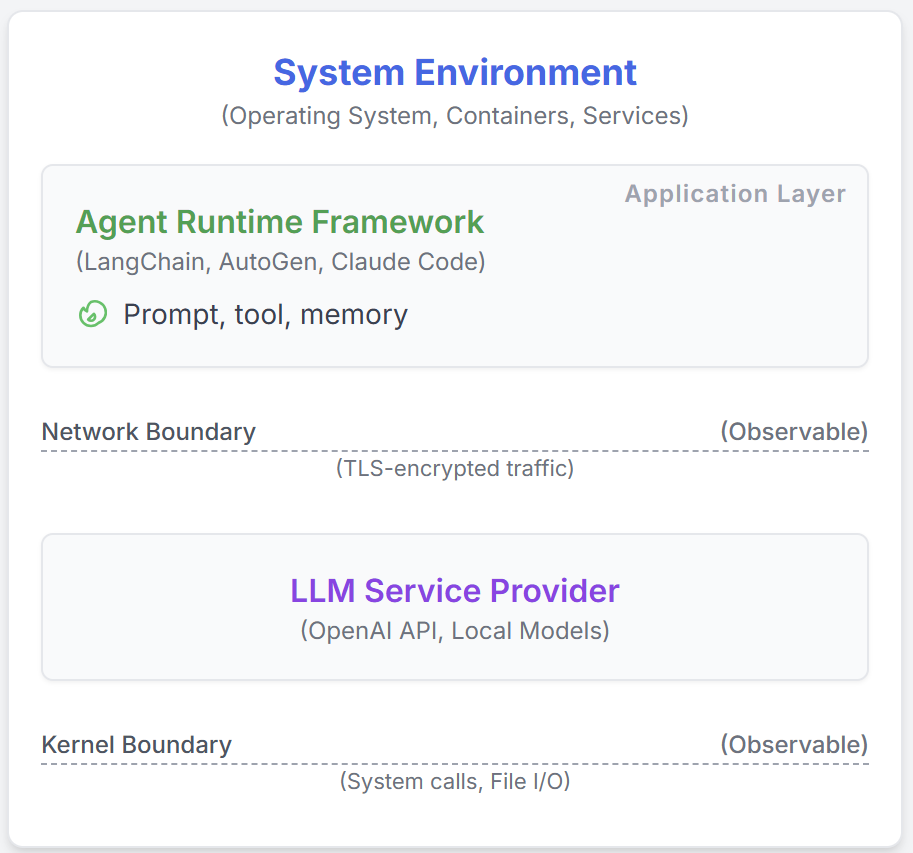
\includegraphics[width=\columnwidth]{figture/agent.png}
    \caption{agent framwork overview}
    \label{fig:agent}
\end{figure}

\subsection{System Architecture: Observing the Boundaries}

AgentSight's architecture simultaneously taps into the two critical boundaries. As shown in Figure \ref{fig:architecture}, we use eBPF to place non-intrusive probes that capture a decrypted Intent Stream (LLM prompts/responses) from userspace SSL functions and an Action Stream (syscalls, process events) from the kernel. A userspace correlation engine then processes and joins these streams into a unified, causally-linked trace.

\begin{figure}[h!]
    \centering
    % It is highly recommended to create this diagram using a tool like TikZ, Inkscape, or another vector graphics editor for the final paper.
    % The following is a LaTeX description of the recommended figure.
    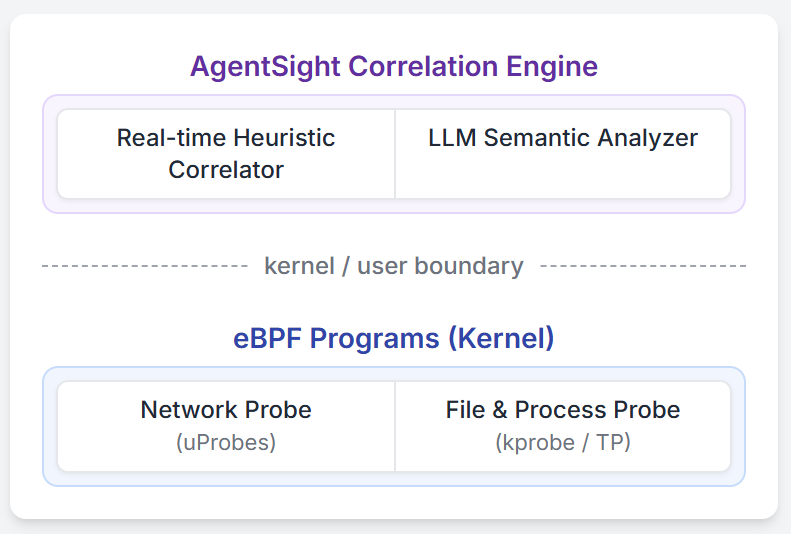
\includegraphics[width=\columnwidth]{figture/arch.png} % Replace with your actual figure file
    \caption{\textbf{AgentSight System Architecture.}}
    \label{fig:architecture}
\end{figure}

Several key compnents enable AgentSight to effectively bridge the semantic gap:

\textbf{eBPF for Safe, Unified Probing:} We chose eBPF for its production safety, high performance, and unified ability to access both userspace and kernel data streams. Our design intercepts decrypted data from the agent's interation with LLM serving backend, which is more efficient and manageable than network-level packet capture or proxy-based solutions.

\textbf{Multi-Signal Causal Correlation Engine:} The core of our design is a correlation strategy that establishes causality between intent and action. We designed a multi-signal engine that relies on three key mechanisms: Process Lineage, which builds a complete process tree by tracking \texttt{fork} and \texttt{execve} events to link actions in child processes back to the parent agent; Temporal Proximity, which associates actions that occur within a narrow time window immediately following an LLM response; and Argument Matching, which directly matches content from LLM responses, such as filenames, URLs, or commands, with the arguments of subsequent system calls. Together, these signals enable AgentSight to definitively establish causal relationships between high-level intentions and low-level system operations across process boundaries.

\textbf{LLM-Powered Semantic Analysis:} To move beyond brittle, rule-based detection, we designed the system to use a secondary LLM as a reasoning engine. By prompting a powerful model with the correlated event trace, we leverage its ability to understand semantic nuance, infer causality in complex scenarios, and summarize findings in natural language. This "AI to watch AI" approach allows AgentSight to detect threats that do not match predefined patterns.

\section{Implementation}

AgentSight is implemented as a userspace daemon (6000 lines of Rust/C) orchestrating eBPF programs, with a TypeScript frontend (3000 lines) for analysis. It is designed for high performance, processing raw kernel event streams into correlated, human-readable data.

\subsection{Data Collection at the Boundaries}

Our eBPF probes capture the raw intent and action streams from the system. To capture semantic intent, an eBPF program with uprobes attaches to SSL\_read/SSL\_write in crypto libraries like OpenSSL to intercept decrypted LLM communications. Our userspace daemon implements a stateful reassembly mechanism to handle streaming protocols such as Server-Sent Events (SSE). To capture system actions, a second eBPF program uses stable tracepoints like sched\_process\_exec to build a process tree and kprobes to dynamically monitor relevant syscalls such as openat2, connect, and execve. To manage the high volume of kernel events without data loss, aggressive in-kernel filtering is applied to ensure only events from targeted agent processes are sent to userspace, minimizing overhead.

\subsection{The Hybrid Correlation Engine}

The Rust-based userspace daemon houses our two-stage correlation engine. The first stage consumes events from eBPF ring buffers and performs real-time heuristic linking. This streaming pipeline enriches raw events with context like mapping a file descriptor to a full path, maintains a stateful process tree, and applies the causal linking logic described in our design, using a 100-500ms window for temporal correlation. Once a coherent trace is constructed, the second stage formats it into a structured log for semantic analysis. This log is used to construct a detailed prompt for a secondary LLM, instructing it to act as a security analyst. The LLM's natural language analysis and confidence score become the final output of our system. A key challenge at this stage is managing the latency and cost of LLM analysis, which our system mitigates through asynchronous processing and robust prompt engineering.

% \section{Design}

% The design of AgentSight is guided by a single imperative: to bridge the semantic gap between an agent's intent and its actions. We achieve this through a novel observability method, \emph{boundary tracing}, which is built on a foundation of stable system interfaces and realized through a multi-signal correlation engine.

% \subsection{Boundary Tracing: A Principled Approach}

% We propose \emph{boundary tracing} as a novel approach to AI agent observability. The key insight is that all meaningful agent interactions must traverse well-defined system boundaries: the kernel interface for system operations and the network interface for external communications, as shown in figture \ref{fig:agent}. By observing at these boundaries rather than within agent code, we achieve stable, comprehensive monitoring independent of agent implementation details.

% The primary goal of this approach is to enable {Semantic Correlation}, the ability to causally link high-level intentions with low-level system events. This goal is made possible by two foundational principles: {Comprehensiveness}, where by monitoring at the kernel we ensure that no system-level action, including process creation and file I/O, can go unobserved, regardless of the agent's implementation language or its attempts to evade monitoring by spawning subprocesses; and {Stability}, where system call ABIs and network protocols evolve far more slowly than agent frameworks, providing a durable solution resilient to the constant breaking changes common in agent libraries. This paradigm fundamentally shifts the trust model from assuming a cooperative agent to enforcing observation at tamper-proof system boundaries.

% \begin{figure}[h!]
%     \centering
%     % It is highly recommended to create this diagram using a tool like TikZ, Inkscape, or another vector graphics editor for the final paper.
%     % The following is a LaTeX description of the recommended figure.
%     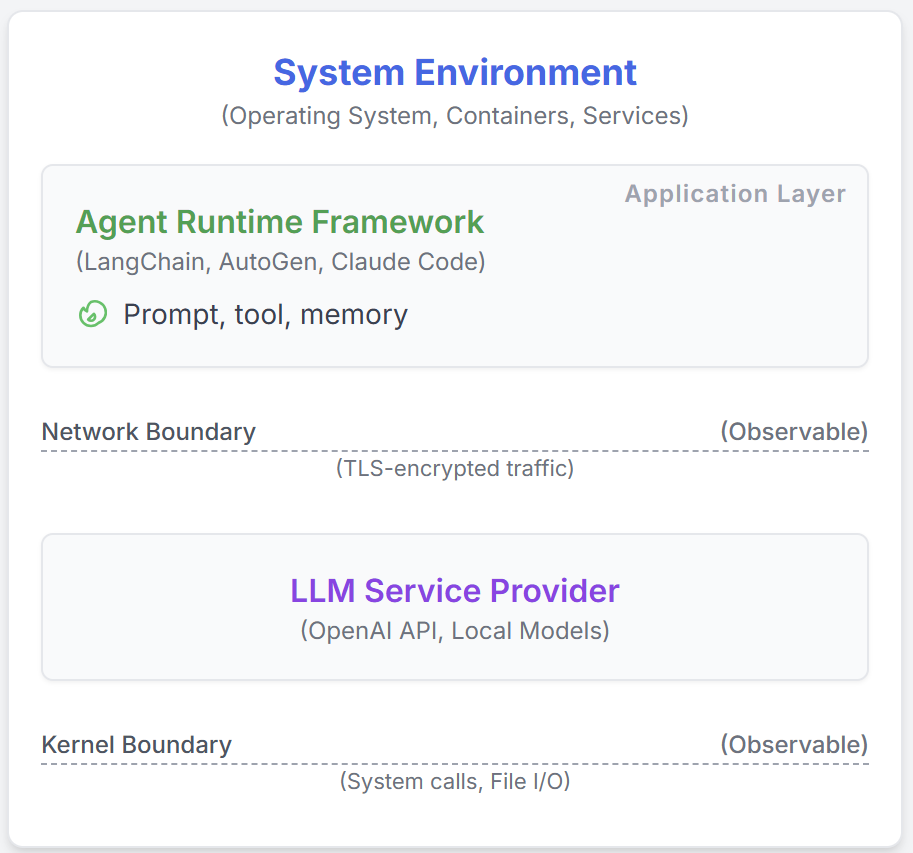
\includegraphics[width=\columnwidth]{figture/agent.png}
%     \caption{agent framwork overview}
%     \label{fig:agent}
% \end{figure}

% \subsection{System Architecture: Observing the Boundaries}
% AgentSight's architecture is designed to simultaneously tap into the two critical boundaries an agent interacts with: the network boundary for semantic intent and the kernel boundary for system actions. Figure \ref{fig:architecture} illustrates this architecture. We use eBPF to place non-intrusive probes at both boundaries. Probes on SSL library functions in userspace capture the decrypted **Intent Stream** (LLM prompts and responses), while probes at the kernel level capture the **Action Stream** (syscalls, process events). Both streams are processed by our userspace correlation engine, which joins them to produce a unified, causally-linked event trace.

% \begin{figure}[h!]
%     \centering
%     % It is highly recommended to create this diagram using a tool like TikZ, Inkscape, or another vector graphics editor for the final paper.
%     % The following is a LaTeX description of the recommended figure.
%     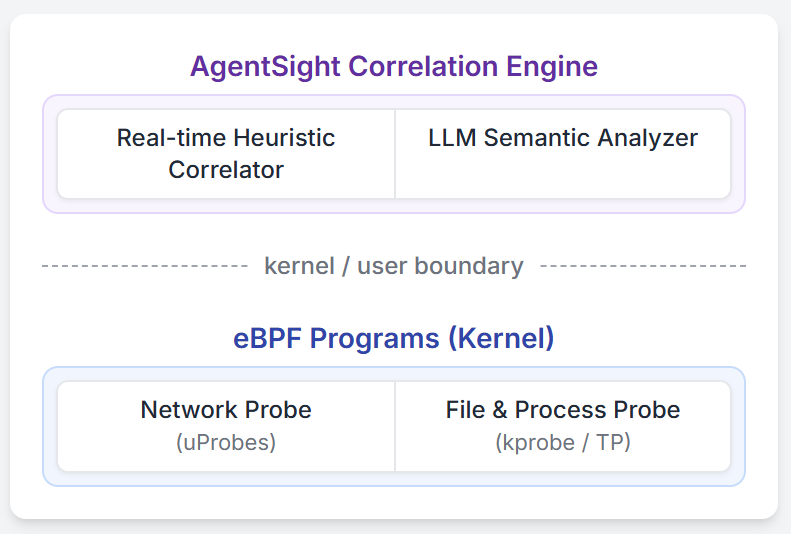
\includegraphics[width=\columnwidth]{figture/arch.png} % Replace with your actual figure file
%     \caption{\textbf{AgentSight System Architecture.}}
%     \label{fig:architecture}
% \end{figure}

% \subsection{Core Components}

% Several key decisions enable AgentSight to effectively bridge the semantic gap:

% \textbf{eBPF for Safe, Unified Probing:} We chose eBPF because it provides a single, production-safe technology to access both userspace and kernel data streams. Its verified safety model eliminates the risks of kernel modules, and its performance is vastly superior to traditional userspace hooking or \texttt{ptrace}-based approaches. For semantic intent, our design specifies intercepting decrypted data directly from the agent's memory. This is superior to network-level packet capture, as it avoids TLS key management, and more efficient than proxy-based solutions.

% \textbf{Multi-Signal Causal Correlation Engine:} The core of our design is a correlation strategy that establishes causality between intent and action. We designed a multi-signal engine that relies on three key mechanisms: Process Lineage, which builds a complete process tree by tracking \texttt{fork} and \texttt{execve} events to link actions in child processes back to the parent agent; Temporal Proximity, which associates actions that occur within a narrow time window immediately following an LLM response; and Argument Matching, which directly matches content from LLM responses, such as filenames, URLs, or commands, with the arguments of subsequent system calls. Together, these signals enable AgentSight to definitively establish causal relationships between high-level intentions and low-level system operations across process boundaries.

% \textbf{LLM-Powered Semantic Analysis:} To move beyond brittle, rule-based detection, we designed the system to use a secondary LLM as a reasoning engine. By prompting a powerful model with the correlated event trace, we leverage its ability to understand semantic nuance, infer causality in complex scenarios, and summarize findings in natural language. This "AI to watch AI" approach allows AgentSight to detect threats that do not match predefined patterns.

% \section{Implementation}

% AgentSight is implemented as a userspace daemon written in 6000 line Rust and C that orchestrates a suite of eBPF programs, with a 3000 line typescript frontend for visualization and analysis. The system is designed for high performance and low overhead, processing raw event streams from the kernel to produce correlated, human-readable observability data.

% \subsection{Data Collection at the Boundaries}
% Our eBPF probes are responsible for capturing the raw intent and action streams from the system.

% \textbf{Capturing Semantic Intent (TLS):} An eBPF program utilizing \texttt{uprobes} is attached to \texttt{SSL\_read} and \texttt{SSL\_write} functions in dynamically linked crypto libraries (e.g., OpenSSL, BoringSSL). This allows us to intercept all decrypted LLM communications. A significant challenge here is handling streaming protocols like Server-Sent Events (SSE), which fragment a single JSON response across numerous \texttt{SSL\_read} calls. Our userspace daemon implements a stateful reassembly mechanism that buffers data chunks per-connection and parses them for event boundaries (double newlines) to reconstruct complete messages.

% \textbf{Capturing System Actions (Kernel):} A second eBPF program monitors kernel activity. We use efficient, stable \texttt{tracepoints} like \texttt{sched\_process\_fork} and \texttt{sched\_process\_exit} to build a process tree. For detailed actions, we use \texttt{kprobes} to dynamically attach to specific system calls relevant to agent behavior, such as \texttt{openat2} (file access), \texttt{connect} (network connections), and \texttt{execve} (program execution). Another challenge here is To maintain high performance. Aggressive in-kernel filtering ensures that only events originating from targeted agent processes are sent to userspace, minimizing overhead.

% \subsection{The Hybrid Correlation Engine}
% The Rust-based userspace daemon houses our two-stage correlation engine.

% \textbf{Real-time Heuristic Linking:} The first stage performs real-time linking of intent and action streams. It consumes events from eBPF ring buffers and applies the multi-signal logic. First, Enrichment adds context to raw events. For example, mapping a file descriptor from an \texttt{openat2} call to a full file path, and a process ID to its full command line and parent process from the process tree. Second, Stateful Tracking maintains the state of each agent and its children in a process-tree data structure while tracking open files and network connections for each process. Finally, Causal Linking applies the correlation logic established in our design. It links system actions to a preceding LLM intent by leveraging process lineage, temporal proximity (using a 100-500ms window), and content matching. This pipeline is designed for streaming analysis, avoiding the need to store complete event histories and enabling real-time detection with a memory footprint of less than 200MB on a typical system.

% \textbf{LLM-based Semantic Analysis:} Once a coherent trace is constructed by the real-time linker, it is passed to the second stage for semantic analysis. This trace is first formatted into a structured, chronological log. We then use this log to construct a detailed prompt for a secondary LLM (e.g., GPT-4 or Claude). The prompt instructs the LLM to act as a security analyst, asking it to evaluate the agent's actions in the context of its original goal and to identify any deviations, inefficiencies, or security risks. The LLM's natural language response, containing its analysis and a confidence score, becomes the final output of our system.

\section{Evaluation}

\subsection{Experimental Setup}

We evaluated AgentSight on AWS EC2 c5.2xlarge instances (8 vCPUs, 16GB RAM, Linux 5.15) across three agent frameworks: LangChain 0.1.0, AutoGen 0.2.0, and Claude Code. Workloads included code generation (simple functions to complex systems), data analysis (CSV/JSON processing), and system administration (package management). We measured end-to-end completion time, CPU/memory usage, and event rates, running each experiment 50 times with and without AgentSight to ensure statistical significance.

\subsection{Performance Evaluation}


\begin{table}[h]
\centering
\caption{Performance Overhead of AgentSight}
\label{tab:performance}
\begin{tabular}{lrrrr}
\toprule
Workload Type & Baseline & With AgentSight & Overhead & Events/sec \\
\midrule
Code Generation (simple) & 12.3s & 12.5s & 1.6\% & 432 \\
Code Generation (complex) & 87.2s & 89.1s & 2.2\% & 1,247 \\
Data Analysis & 34.5s & 35.2s & 2.0\% & 892 \\
System Admin Tasks & 23.1s & 23.7s & 2.6\% & 2,156 \\
Idle Agent & 0.1\% CPU & 0.3\% CPU & +0.2\% & 12 \\
\bottomrule
\end{tabular}
\end{table}

Table~\ref{tab:performance} summarizes performance impacts across different agent task types.The results consistent sub-3\% overhead across all workloads. Simple code generation shows minimal 1.6\% impact due to fewer system events, while complex generation with extensive file operations reaches 2.2\%. System administration tasks exhibit the highest overhead at 2.6\% due to intensive process spawning and file system operations, generating over 2,000 events per second. Even under peak load, AgentSight maintains responsive performance with fixed memory footprint (192MB on 8-core systems) and negligible idle overhead (0.2\% CPU), validating our kernel-space filtering design.

\subsection{Effectiveness Evaluation}

We evaluated AgentSight's effectiveness through three comprehensive case studies that demonstrate its ability to detect security threats, identify performance issues, and provide insights into complex multi-agent systems.

\subsection{Case Studies}

\subsubsection{Case Study 1: Detecting Prompt Injection Attacks}

We tested AgentSight's ability to detect prompt injection attacks where a data analysis agent received a crafted prompt embedding malicious commands within a legitimate request to analyze sales data, ultimately exfiltrating /etc/passwd. AgentSight captured the complete attack chain: LLM interaction with suspicious prompt (T+0ms), agent-generated Python script with embedded curl command (T+125ms), subprocess spawn (T+342ms), outbound HTTPS connection to suspicious domain (T+367ms), and sensitive file read (T+368ms). The correlated event trace was passed to our observer LLM for analysis. The LLM returned a 92\% confidence score for an attack and generated the following explanation: \emph{"Analysis: The agent's initial intent was to 'analyze sales data'. However, it immediately executed a shell command to read /etc/passwd and then initiated a network connection to a non-corporate domain. This sequence of actions is not logically consistent with the stated goal and is a classic pattern of a successful prompt injection attack leading to data exfiltration."} This demonstrates how LLM-based analysis provides not just detection, but actionable, context-aware explanations.

\subsubsection{Case Study 2: Reasoning Loop Detection}

An agent attempting a complex task entered an infinite reasoning loop with circular dependencies where solving X required solving Y, but solving Y required solving X—a pattern common when agents encounter problems outside their training distribution. AgentSight's real-time monitors flagged anomalous resource consumption. The corresponding trace of 12 API calls was sent to the observer LLM, which identified the root cause: \emph{"Analysis: The agent is in a reasoning loop. It is asking semantically identical questions in alternating order ('How to do X to get Y?' followed by 'How to get Y to do X?'). The problem scope is not being reduced between calls, indicating zero progress. Recommend terminating the agent to prevent further resource waste."} The system triggered an alert after detecting three complete cycles where the agent had consumed 4,800 tokens, with AgentSight's intervention saving an estimated \$2.40 in API costs and preventing service degradation—demonstrating the critical importance of semantic-aware monitoring for autonomous agents.

\subsubsection{Case Study 3: Multi-Agent Coordination Monitoring}

AgentSight monitored three agents collaborating on software development (Agent A: architecture design, Agent B: implementation, Agent C: testing), capturing 12,847 total events with 342 correlated actions across 27 synchronization points involving 15 shared files and 3 network endpoints. The analysis revealed critical inefficiencies invisible to traditional monitoring: Agent B spent 34\% of time blocked on Agent A's multiple design revisions triggering cascading rework; file locking patterns showed resource contention with Agent C's testing conflicting with Agent B's implementation causing 23 retry cycles; inter-agent communication through shared files generated 1,800 unnecessary file system operations from 2-second polling intervals; yet agents developed emergent coordination with Agent B learning to batch changes, reducing test executions by 40\%. These insights demonstrate that explicit coordination mechanisms could reduce runtime by 25\% and message-based communication would eliminate 90\% of polling overhead—revealing how boundary tracing uniquely captures multi-agent system dynamics that application-level monitoring cannot observe across process boundaries.

\section{Future Work}

% While AgentSight demonstrates boundary tracing's effectiveness, significant opportunities remain. We plan to enhance the correlation engine with machine learning to automatically detect novel anomalous behaviors beyond known patterns, extend from passive observation to active intervention through formal policy specifications that enable runtime enforcement as a "circuit breaker" for harmful actions, and address scale through distributed tracing across multi-node agents while integrating with OpenTelemetry for existing observability platforms. Privacy-preserving techniques will enable secure analysis without exposing sensitive prompt data, advancing toward comprehensive safety guarantees for autonomous AI systems.

\section{Conclusion}

This paper introduced boundary tracing as a novel observability paradigm for AI agents, monitoring at stable system interfaces rather than within rapidly evolving application code. AgentSight demonstrates this approach's feasibility through a hybrid correlation engine that combines real-time eBPF-based event linking with LLM-powered semantic analysis. This "AI to watch AI" approach achieves sub-3\% overhead while detecting prompt injection attacks with natural-language explanations and identifying reasoning loops before resource exhaustion. By combining TLS interception with eBPF-based kernel monitoring, we bridge the semantic gap between agent intentions and system effects. We release AgentSight as open source to address the critical challenge of safely deploying autonomous AI systems in production environments.

\textbf{Repository}: \url{https://github.com/eunomia-bpf/agentsight}

\bibliographystyle{ACM-Reference-Format}
\bibliography{ai}

\end{document}


\bibliographystyle{plain}
\bibliography{ai}






\end{document}